\documentclass[xcolor=dvipsnames,aspectratio=169]{beamer}

% INCLUSIÓN DOS PAQUETES IMPRESCINDIBLES DE IDIOMA E CODIFICACIÓN DE CARACTERE.
\usepackage[T1]{fontenc}
\usepackage[english]{babel}
\usepackage[utf8]{inputenc}
\usepackage{csquotes}

%ACRONYMS para engadir un glosario de acronimos automatizado
% \usepackage[acronyms,nonumberlist,nopostdot,nomain,nogroupskip]{glossaries}
% \input{./acronyms.tex}

% PAQUETES PARA FIGURAS E GRAFICOS
\usepackage{graphicx}
%   \usepackage[pdftex]{graphicx}
  \usepackage{epstopdf}
   \graphicspath{{./img/}}
  % and their extensions so you won't have to specify these with
  % every instance of \includegraphics
   \DeclareGraphicsExtensions{.eps,.pdf,.png,.jpg}   
\usepackage{subfigure}
\usepackage{caption}

%Tikz plots
\usepackage{tikz}
\usepackage{tikzscale}
\usetikzlibrary{plotmarks,patterns,decorations.pathreplacing,backgrounds,calc,arrows,arrows.meta,spy,matrix,backgrounds}
\newcommand{\tikzmark}[1]{\tikz[overlay,remember picture] \UE (#1) {};}
\newcommand{\DrawBox}[4][]{%
    \tikz[overlay,remember picture]{%
        \coordinate (TopLeft)     at ($(#2)+(-0.4em,1.6em)$);
        \coordinate (BottomRight) at ($(#3)+(0.4em,-1.0em)$);
        %
        \path (TopLeft); \pgfgetlastxy{\XCoord}{\IgnoreCoord};
        \path (BottomRight); \pgfgetlastxy{\IgnoreCoord}{\YCoord};
        \coordinate (LabelPoint) at ($(\XCoord,\YCoord)!0.5!(BottomRight)$);
        %
        \draw [red,#1] (TopLeft) rectangle (BottomRight);
        \UE [below, #1, fill=none, fill opacity=1] at (LabelPoint) {#4};
    }
}
\usepackage{pgfplots}
\pgfplotsset{compat=newest}
\pgfplotsset{plot coordinates/math parser=false}
\usepgfplotslibrary{patchplots,groupplots}

% OUTROS PAQUETES DE USO COMUN. HOXE EN DIA OS COMPILADORES SON TAN RAPIDOS QUE EU METO TODOS SEMPRE
% \usepackage{float}
% \usepackage{ucs} 
% \usepackage{subcaption}
\usepackage{psfrag}
\usepackage{verbatim}
\usepackage{amsmath}
\usepackage{amsfonts} 
\usepackage{amssymb} 
\usepackage{amsthm}
\usepackage{pifont}
\usepackage{array}
\usepackage{listings}
\usepackage{stfloats}
\usepackage{algorithm} 
\usepackage{algorithmic} 
\usepackage{url} 
\usepackage{enumerate}
\usepackage{multirow}
\usepackage{wasysym}


% DECLARACION DAS FONTES DA UVIGO
\usepackage[sfdefault]{roboto}
\usepackage{librebaskerville}
\setbeamerfont{title}{family=\librebaskerville,size=\Huge}
\setbeamerfont{subtitle}{family=\librebaskerville,size=\large}
% IMPORTANTE: a fonte 'campus' non queda ben para títulos de papers academicos,ç
% pero se de verdade se desexa empregar, seguir os seguintes pasos
% 1) Instalar o comando otftotfm en linux
% 2) sudo otftotfm -a -e texnansx campus_bold.otf CampusBold
% 3) asegurarse que o ficheiro auxiliar ./EETtemplateFiles/fonts/T1CampusBold.df está no directorio de traballo
% 4) descomentar a liña abaixo e comentar a liña que lle asigna librebaskerville arriba
\input{EETtemplateFiles/fonts/T1CampusBold.df}
\setbeamerfont{title}{family=\fontfamily{CampusBold},size=\Huge}

% DETLARACIÓN DO TEMA A USAR
% 
% ESTES TEMAS TEÑEN CABECEIRAS MOI GRANDES
% \usetheme{Berkeley} %large titlebar w/side dossier
% \usetheme{PaloAlto} 
% \usetheme{Copenhagen} %large titlebar w/2 side index
% \usetheme{Antibes} %large titlebar w/tree
% \usetheme{Singapore} %large titlebar w/balls evanescent
% \usetheme{Berlin} %large titlebar w/balls solid
% \usetheme{Dresden} %same as above with different color boxing
% \usetheme{Rochester} %large tittle-only titlebar
% ESTES TEMAS TEÑEN CABECEIRAS MEDIANAS
% \usetheme{CambridgeUS} %title titlebar w/current section
% \usetheme{Malmoe} %title titlebar w/current section Copenhagen style
% \usetheme{Madrid} %title titlebar w/page counter footer
% ESTES TEMAS TEÑEN CABECEIRAS DELGADAS
% \usetheme{Frankfurt} %small titlebar w/ progress balls
% \usetheme{metropolis} %metal
% ESTES TEMAS NON TEÑEN CABECEIRA DE COR, PERO SI TITULO SOBRE BRANCO
% \usetheme{Boadilla} %sombras e decoracion
\usetheme{Pittsburgh} %rectangulos planos
% ESTES TEMAS TEÑEN INDICES OU INFO NUNHA BARRA LATERAL GRANDE
% \usetheme{Goettingen} %right dossier evanescent
% \usetheme{Marburg} %right dossier fading to black
% \usetheme{Bergen} %notebook

%aspect modifiers
\useinnertheme{circles} %this makes item lists nicer
% \useoutertheme{infolines} %toggle thin info borders


% DECLARACIÓN DA COMBINACIÓN DE CORES A USAR. SE NON SE ESPECIFICA NADA TOMA A DEFINIDA POR DEFECTO
\definecolor{EETblue}{HTML}{0094e0} % a mate dark blue
\usecolortheme[named=EETblue]{structure} % EET UVigo blue
% outros temas de cores de beamer
% \usecolortheme{seagull} %makes title boxes gray color with blackr
% \usecolortheme{spruce} %makes title boxes pastel blue - gray color
% cores internos (items)
% \usecolortheme[named=Red]{structure} 
% \usecolortheme[named=Green]{structure} 
% \usecolortheme[named=OliveGreen]{structure} 
% \usecolortheme[named=PineGreen]{structure} 
% \usecolortheme[named=TealBlue]{structure} 
% \usecolortheme[named=SeaGreen]{structure}
% \usecolortheme[RGB={00,78,135}]{structure} % a dark cobalt blue 
% \usecolortheme[RGB={155,0,20}]{structure} % a slighlty darkened mate red

% MODIFICACIONS DAS CORES PARA A PAXINA DE TITULO SIMILAR Á OFICIAL
\setbeamercolor*{title}{use=structure,fg=structure.bg, bg=structure.fg}  
\setbeamercolor*{subtitle}{use=structure,fg=white}  
\setbeamercolor*{author}{use=structure,fg=structure.fg}
% \setbeamercolor*{institute}{use=structure,fg=structure.fg}
\setbeamercolor*{date}{use=structure,fg=structure.fg}
\setbeamertemplate{frametitle}[default][left]

% MODIFICACIONS DA SIDEBAR E FOOTLINE PARA INCLUIR AS IMAXES CORPORATIVAS.
\setbeamertemplate{footline}[text line]{%
  \parbox{\linewidth}{
    %ESTE TEXTO DA FOOTLINE PODESE MODIFICAR A GUSTO -----------------------------------------
    \insertshorttitle\hfill\insertshortauthor\hfill\insertpagenumber / \inserttotalframenumber
    %----------------------------------------------------------------------------------------
    \hfill
  
\includegraphics[width=.15\paperwidth,trim={0 2.5cm 3.5cm .75cm},clip]{EETtemplateFiles/img/Logotipo_ESCOLA.pdf}\vspace*{2pt}}}
\setbeamersize{sidebar width left = .10\paperwidth}
\setbeamertemplate{sidebar canvas left}{}
\setbeamertemplate{sidebar left}{%
  \vspace*{\fill}
  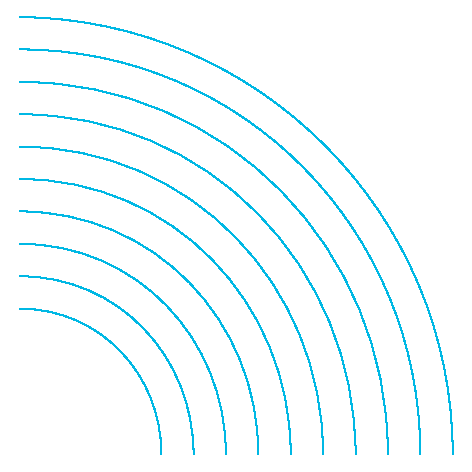
\includegraphics[width=.15\paperwidth,height=.15\paperwidth]{EETtemplateFiles/img/Simbolo_ESCOLA.pdf}\\
  
\includegraphics[width=.15\paperwidth,trim={.4cm .5cm .4cm 2.25cm},clip]{EETtemplateFiles/img/Logotipo_ESCOLA.pdf}
  \vspace*{-11pt}%
}

% MATH SYMBOLS

\newcommand{\field}[1]{\mathbb{#1}}

\DeclareMathOperator{\atan}{atan}
\DeclareMathOperator{\acos}{acos}
\DeclareMathOperator{\asin}{asin}

% \newcommand{\mb}[1]{\mathbf{#1}}


\newcommand{\Hb}{\mathbf{H}}
\newcommand{\Sb}{\mathbf{\boldsymbol{\Sigma}}}
\newcommand{\Sm}{\mathbf{S}}
\newcommand{\U}{\mathbf{U}}
\newcommand{\F}{\mathbf{F}}
\newcommand{\V}{\mathbf{V}}
\newcommand{\A}{\mathbf{A}}
\newcommand{\B}{\mathbf{B}}
\newcommand{\Cb}{\mathbf{C}}
\newcommand{\D}{\mathbf{D}}
% \newcommand{\E}{\mathbf{E}}
\newcommand{\Gb}{\mathbf{G}}
\newcommand{\T}{\mathbf{T}}
\newcommand{\I}{\mathbf{I}}
\newcommand{\Y}{\mathbf{Y}}
\newcommand{\M}{\mathbf{M}}
\newcommand{\N}{\mathbf{N}}
\newcommand{\W}{\mathbf{W}}
\newcommand{\Z}{\mathbf{Z}}
\newcommand{\R}{\mathbf{R}}
\newcommand{\K}{\mathbf{K}}
\newcommand{\X}{\mathbf{X}}
\newcommand{\Pb}{\mathbf{P}}
\newcommand{\Lb}{\mathbf{L}}
\newcommand{\Phib}{\mathbf{\boldsymbol{\Phi}}}
\newcommand{\Upsb}{\mathbf{\boldsymbol{\Upsilon}}}
\newcommand{\Delb}{\mathbf{\boldsymbol{\Delta}}}
\newcommand{\Xib}{\mathbf{\boldsymbol{\Xi}}}
\newcommand{\Q}{\mathbf{Q}}
% \newcommand{\D}{\mathbf{D}}
\newcommand{\one}{\mathbf{1}}
\newcommand{\zero}{\mathbf{0}}
\newcommand{\Rm}{\mathbf{R^{-1}}}
\newcommand{\LL}{\mathbf{\boldsymbol{\Lambda}}}
\newcommand{\J}{\mathbf{J}}

\newcommand{\ab}{\mathbf{a}}
\newcommand{\bb}{\mathbf{b}}
\newcommand{\cc}{\mathbf{c}}
\newcommand{\dd}{\mathbf{d}}
\newcommand{\e}{\mathbf{e}}
\newcommand{\f}{\mathbf{f}}
\newcommand{\g}{\mathbf{g}}
\newcommand{\h}{\mathbf{h}}
\newcommand{\m}{\mathbf{m}}
\newcommand{\n}{\mathbf{n}}
\newcommand{\pp}{\mathbf{p}}
\newcommand{\q}{\mathbf{q}}
\newcommand{\rr}{\mathbf{r}}
\newcommand{\s}{\mathbf{s}}
\newcommand{\uu}{\mathbf{u}}
\newcommand{\vv}{\mathbf{v}}
\newcommand{\w}{\mathbf{w}}
\newcommand{\x}{\mathbf{x}}
\newcommand{\y}{\mathbf{y}}
\newcommand{\z}{\mathbf{z}}
\newcommand{\al}{\mathbf{\boldsymbol{\alpha}}}
\newcommand{\vmu}{\mathbf{\boldsymbol{\mu}}}
\newcommand{\vlambda}{\mathbf{\boldsymbol{\lambda}}}
\newcommand{\vphi}{\mathbf{\boldsymbol{\phi}}}
\newcommand{\vrho}{\mathbf{\boldsymbol{\rho}}}
\newcommand{\vups}{\mathbf{\boldsymbol{\upsilon}}}

\newcommand{\rank}{\textnormal{rank}}
% \newcommand{\trace}{\textnormal{trace}}
\newcommand{\exptr}{\textnormal{exptr}}
\newcommand{\tr}{\textnormal{tr}}
\newcommand{\vstack}{\textnormal{vec}}
\newcommand{\diag}{\textnormal{diag}}
%  |x>
\newcommand{\ket}[1]{\left\vert#1\right\rangle}
%  <x|
\newcommand{\bra}[1]{\left\langle#1\right\vert}
%  <x|y>
\newcommand{\braket}[2]{\left< #1 \vphantom{#2}\,
                        \right\vert\left.\!\vphantom{#1} #2 \right>}
%  <x|a|y>
\newcommand{\sandwich}[3]{\left< #1 \vphantom{#2 #3} \right|
                          #2 \min\left(\vphantom{#1 #2} #3 \right>}

\newcommand{\pd}[2]{\frac{\partial #1}{\partial #2}}
%  d/dt
\newcommand{\ddt}{\frac{d}{dt}}
%  D/Dx
\newcommand{\pdd}[1]{\frac{\partial}{\partial#1}}
%  |x|
\newcommand{\abs}[1]{\left\vert#1\right\vert}
%  k_{x}
\newcommand{\kv}[1]{\mathbf{k}_{#1}}
%  \textnormal{E}_{domain of integration}{variable}
\newcommand{\Ex}[2]{{\mathbb{E}_{#1}\left[#2\right]}}
\newcommand{\CEx}[3]{{\mathbb{E}_{#1}\left[#2|#3\right]}}
\newcommand{\CInf}[3]{{\textnormal{I}\left(#1;#2|#3\right)}}
\newcommand{\Inf}[2]{{\textnormal{I}\left(#1;#2\right)}}
\newcommand{\CEnt}[2]{{\textnormal{H}\left(#1|#2\right)}}
\newcommand{\Ent}[1]{{\textnormal{H}\left(#1\right)}}
\newcommand{\dCEnt}[2]{{\textnormal{h}\left(#1|#2\right)}}
\newcommand{\dEnt}[1]{{\textnormal{h}\left(#1\right)}}

\newcommand{\cmark}{\ding{51}}%
\newcommand{\xmark}{\ding{55}}%
\newcommand\Tau{\mathcal{T}}
%Figure and format fixes


\renewcommand{\figurename}{Fig.}
\newcommand{\PESrule}{\noindent\rule{.57\columnwidth}{0.1mm}}

% A command to make itemized table contents

%theroem environments
% If using amsthm package, we need to delete these theorems before giving them our own definition. does not work for theorem
% \let\theorem\relax
\let\definition\relax
\let\lemma\relax
\let\corollary\relax
\let\example\relax
%
% \newtheorem{theorem}{Theorem}
\newtheorem{definition}{Definition}
\newtheorem{lemma}{Lemma}
\newtheorem{corollary}{Corollary}
\newtheorem{conjecture}{Conjecture}
\newtheorem{example}{Example}
\theoremstyle{plain}
\newtheorem{remark}{Remark}
\newtheorem{proposition}{Proposition}
   \newtheorem{homework}{Homework}

%Colors
   \definecolor{blueH3}{rgb}{0,.5,1}
   \definecolor{blueH2}{rgb}{0,0.25,0.75}
   \definecolor{blueH1}{rgb}{0,0,0.5}   
   \definecolor{grayOldText}{rgb}{.5,.5,.5}
   \definecolor{VCobalt}{HTML}{005682}
   \definecolor{TZTeal}{HTML}{008080}
   \definecolor{TZTealfaded}{HTML}{F0FFFF}
   \definecolor{KYJade}{HTML}{008151}
   \definecolor{ARust}{HTML}{a10000}
   \definecolor{FFucsia}{HTML}{7000c3}   
   \definecolor{TAMustard}{HTML}{a1a100}
   \definecolor{Tangerine}{HTML}{d45500}
   
   %%%%%%%%%%%%%%%%%%%%%%%%%%%%%%%%%%%%%%%%%%%%%%%%%%%%%%%%%%%%%%%%%
%% The following definitions are to extend the LaTeX algorithmic 
%% package with SWITCH statements and one-line structures.
%% The extension is by 
%%   Prof. Farn Wang 
%%   Dept. of Electrical Engineering, 
%%   National Taiwan University. 
%% 
\newcommand{\SWITCH}[1]{\STATE \textbf{switch} (#1)}
\newcommand{\ENDSWITCH}{\STATE \textbf{end switch}}
\newcommand{\CASE}[1]{\STATE \textbf{case} #1\textbf{:} \begin{ALC@g}}
\newcommand{\ENDCASE}{\end{ALC@g}}
\newcommand{\CASELINE}[1]{\STATE \textbf{case} #1\textbf{:} }
\newcommand{\DEFAULT}{\STATE \textbf{default:} \begin{ALC@g}}
\newcommand{\ENDDEFAULT}{\end{ALC@g}}
\newcommand{\DEFAULTLINE}[1]{\STATE \textbf{default:} }
%% 
%% End of the LaTeX algorithmic package extension.

\newcounter{MYtempeqncnt}


%%%%%%%%%%%%%%%%%%%%%%%%%%%%%%%%%%%%%%%
% Commands to recall text later
%%%%%%%%%%%%%%%%%%%%%%%%%%%%%%%%%%%%%%%
\makeatletter
\newcommand\remembertext[2]{% #1 is a key, #2 is the text
  \immediate\write\@auxout{\unexpanded{\global\long\@namedef{mytext@#1}{#2}}}%
  #2%
}
%
\newcommand\recalltext[1]{%
  \ifcsname mytext@#1\endcsname
    \@nameuse{mytext@#1}%
  \else
    ``??''
  \fi
}

%%%%%%%%%%%%%%%%%%%%%%%%%%%%%%%%%%%%%%%%%%%%%%%%%%%%%%%%%%%%%%%%%%%%%%%%%%%%%%%%%%
%%% Paolo Casari: macros for automating section titling and comment formatting %%%
%%%%%%%%%%%%%%%%%%%%%%%%%%%%%%%%%%%%%%%%%%%%%%%%%%%%%%%%%%%%%%%%%%%%%%%%%%%%%%%%%%
\newcounter{myequationcnt}

\newcounter{rcnt}
\newcounter{ccnt}

\newcommand{\newreviewernopagebreak}[1]{\vspace{5em} \setcounter{ccnt}{0}\section*{\normalsize Comments of #1}\vspace{4mm}}

\newcommand{\ThisIsTheEditorNoPageBreak}{\setcounter{ccnt}{0}\section*{\Large Comments of the Editor}\vspace{3mm}}
\newcommand{\ThisIsTheEditor}{\clearpage \ThisIsTheEditorNoPageBreak}
\newcommand{\ThisIsANewReviewerNoPageBreak}[1]{\vspace{5em} \refstepcounter{rcnt}\label{r#1}\setcounter{ccnt}{0}\section*{\Large Comments of Reviewer \arabic{rcnt}}\vspace{3mm}}
\newcommand{\ThisIsANewReviewer}[1]{\clearpage\vspace{-5em} \ThisIsANewReviewerNoPageBreak{#1}}

\newcommand{\edcomment}[1]{
\begin{tcbremark}
\color{VCobalt}
    \refstepcounter{ccnt}\label{e\arabic{ccnt}}\noindent\textbf{\boldmath\emph{Comment E.\arabic{ccnt}:}} #1\vspace{0.2cm}
\end{tcbremark}
}
\newcommand{\refedcomment}[1]{E.\ref{e#1}}

\newcommand{\revcomment}[1]{
\begin{tcbremark}
\color{VCobalt}
\refstepcounter{ccnt}\label{r\arabic{rcnt}c\arabic{ccnt}}\noindent\textbf{\boldmath\emph{Comment \arabic{rcnt}.\arabic{ccnt}:}} #1\vspace{0.2cm}
\end{tcbremark}
}
\newcommand{\refrevcomment}[2]{\ref{r#1}.\ref{r#1c#2}}

% \newcommand{\ouranswer}[1]{\noindent\emph{Answer:} #1\vspace{0.6cm}}
% \newcommand{\citepap}[1]{\vspace{0.33cm}\begin{minipage}{0.05\textwidth} $\phantom{A}$  \end{minipage}\begin{minipage}{0.85\textwidth}\renewcommand{\baselinestretch}{1.15}\small \emph{#1} \end{minipage}\vspace{0.3cm}}

\newlength{\ansspace}
\addtolength{\ansspace}{0.6cm}
\newcommand{\ansbreak}{\vspace{\ansspace}}

\newlength{\stdleftskip}
\addtolength{\stdleftskip}{\leftskip}
\newlength{\stdrightskip}
\addtolength{\stdrightskip}{\rightskip}
\newlength{\citeskip}
\addtolength{\citeskip}{2em}
\newcommand{\oldbaselinestretch}{1.5}

\newcommand{\setcitepapskip}{%
    \leftskip\citeskip %
    \rightskip\citeskip %
    \renewcommand{\baselinestretch}{1.15}\small%
    \vspace{0.6em}%
    \noindent%
}

\newcommand{\resetLRmargins}{%
    \leftskip\stdleftskip %
    \rightskip\stdrightskip %
    \renewcommand{\baselinestretch}{\oldbaselinestretch}\normalsize %
    \vspace{0.6em}
}

\newcommand{\emans}{\emph{Answer:\ }}


%---------------
% LIMIAR
%---------------
%configuracion de opcions de beamer persoais, pero alleas ao estilo

% COMANDO QUE INTRODUCE UNHA DIAPOSITIVA CUN ÍNDICE NO QUE APARECEN VELADAS TÓDALAS SECCIÓNS MENOS A ACTUAL. ÚTIL PARA INTRODUCIR OS TÍPICOS ÍNDICES INTERMEDIOS.
\newcommand{\Inter}{\frame{\tableofcontents[currentsection]}}
\newcommand{\inter}{\frame{\tableofcontents[currentsection,currentsubsection]}}

% Pes de imaxe
\renewcommand{\figurename}{Fig.}
\addto\captionsenglish{\renewcommand{\figurename}{Fig.}}
\setbeamertemplate{caption}[numbered]

%ESTE PAQUETE PERMITE POÑER A BIBLIOGRAFIA AO PE DE PAXINA CON CONFIGURACIONS ESTETICAS PERSOAIS
% \usepackage[style=ieee,doi=false,isbn=false,url=true,backend=bibtex]{biblatex}
% \bibliography{./bibliografia.bib}
% \newrobustcmd*{\footfullcitenomark}{%
%   \AtNextCite{%
%     \let\thefootnote\relax 
%     \let\mkbibfootnote\mkbibfootnotetext
%     }%
%   \footfullcite}

%paquete para engadir notas de guion ao pdf
\usepackage{pgfpages}
% \setbeameroption{show only notes} 
% \setbeameroption{show notes}
% \setbeameroption{show notes on second screen=right}
% DATOS DO DOCUMENTO
\title{Advanced Communication Systems} 
\subtitle{Part 2: Multi-user Communications}
\author[FGC]{Felipe G\'omez Cuba}
\institute[XX]{
\begin{columns}[T]
\begin{column}{9cm}\centering
Despacho 204\\
Titorías: Lun-Xov 15:00-16:30\\
(En caso de confinamento: videochamada a calquera horario acordado)\\
  \texttt{gomezcuba@gts.uvigo.es}\\
\end{column}
\end{columns}
}

\date{}

\begin{document}

% Diapositiva co título
%\frame[plain]{\titlepage}%the ``classic'' beamer cover pageç

\frame{\frametitle{\\}%generate top bar, but blank line as tittle
\titlepage
}%approximation to the ``GPSC ppt'' cover page, but with central beamer title

% \frame{\tableofcontents}
% \note[itemize]{%itemized notes are special ``note'' slides that beamer can append to the pdf or not, depending on a boolean toggle option
% \item Introduce yourself
% \item In this work we studied blablabla.
% }

\frame[allowframebreaks]{\frametitle{Presentation of Contents}
% \begin{itemize}
%  \item \textbf{Motivation}: to apply optimization and MIMO to achieve high performance multi-user communications.\\ \ \\
%  \item 
 \textbf{Outline of the Contents (15h)}:
     \begin{enumerate}
        \item Recap of single-user Information Theory from CDA (self study)
%         \begin{description}
%             \item[$\dag$] definitions: entropy
%             \item[$\dag$] usual random variables and examples 
%             \item[$\dag$] joint entropy and conditional entropy, chain rule
%             \item[$\dag$] joint entropy and vectors of random variables, typical examples
%             \item[$\dag$] diferential entropy continuous r.v.
%             \item[$\dag$] mutual information
%             \item[$\dag$] properties of entropy and mut inf. multiple variables. chain rule.
%             \item[$\dag$] notion of capacity, capacity of BSC
%             \item[$\dag$] capacity of the real AWGN channel
%             \item[$\dag$] real RF continuous time channel -> DEC -> capacity of the complex AWGN channel 
%             \item[$\dag$] lessons of the capacity proof: error pobability as low as desired as codeword size -> inf, sup Mut Inf over space of all pdfs, Gaussian achieves
%             \item[$\dag$] importance of the ML detector
%             \item[$\dag$] bits per channel use vs bps, bandwidth, spectral efficiency, energy efficiency, DoF...
%             %___________________________________s2
%             \item[$\dag$] mutual information of N-QAM, AMC to approximate capacity in practice, ML with QAM (decisor in SISO, sphere decoding in MIMO)
%             \item[$\dag$] suboptimal detectors in MIMO
%             \item[$\dag$] fading, OFDM with per-subcarrier MIMO
%             \item[$\dag$] undefined capacity in the classic sense, ergodic (emphasis OFDM) and outage (emphasis narrowband) capacity
%          \end{description}
        
        \item Multiple Access Channel and receiver (3.5h)
%         \begin{description}
%             \item[$\dag$]  concept of multi-dimensional rate vector
%             \item[$\dag$]  representing the newtwork in a graph
%             \item[$\dag$]  cut set bound method
%             \item[$\dag$]  concept of rate-region, via union of all cut set bounds
%             \item[$\dag$]  one-user cut is known capacity result
%             \item[$\dag$]  each multi user cut stems from a chain rule 
%______________________________s2
%             \item[$\dag$]  reminder of MIMO capacity and comparison of MIMO channel with cut-set bound.
%             \item[$\dag$]  achievable rate regions based on orthogonal resource division: TDMA, FDMA, CDMA and OFDMA
%             \item[$\dag$]  fixed instantaneous power vs. average power constraint vs resource allocation.
%             \item[$\dag$]  capacity achieving scheme based on non-orthogonal detection
%             \item[$\dag$]  concept of successive decoding (TIN) as interpretation of the chain rule
%             \item[$\dag$]  slow Fading, joint outage analysis and wideband optimal orthogonal
%             \item[$\dag$]  Fast Fading, averaging the cut set bound and FDMA no longer has max sum rate
%             %_____________________________________s3
%             \item[$\dag$]  Concept of individual and joint error probability
%             \item[$\dag$]  in orthogonal cases each user signal is independent and single-user decoders are ``optimal''
%             \item[$\dag$]  multiuser is harder than MIMO because of no joint encoding and asymmetries
%             \item[$\dag$]  joint MAP detector minimizes Pe
%             \item[$\dag$]  ML detector 
%             \item[$\dag$]  linear MUD [MMSE, ZF, MF]
%             \item[$\dag$]  practical SIC with QAM and independent user detector is suboptimal but faster
%             \item[$\dag$]  non-linear MUD: DF as a non-linear addition to matrix inversion Taylor method
%             \item[$\dag$]  non-linear MUD: IDD and MAP decoding schemes
%         \end{description}
        
        \item Broadcast Channel and transmitter (3.5h)
%         \begin{description}
%             \item[$\dag$] Common vs individual messages: tv broadcast vs cellular
%             \item[$\dag$] SISO, concept of a shared power constraint
%             \item[$\dag$] Single user cut bounds with full power
%             \item[$\dag$] Corner case: shared rate achievable by both users
%             \item[$\dag$] Extension to superposition code and SIC, interpreted as $P_1$ common message + $P_2$ dedicated
%             \item[$\dag$] Explanation of NOMA
%             \item[$\dag$] Dual MAC channel Theorems
%             \item[$\dag$] Interpretation of the BC capacity region as a convex optimization
%             \item[$\dag$] Interpretation as convex-hull of dual MAC channels
%             \item[$\dag$] MIMO special case with $n_t>U$, orthogonal channels. Motivation of precoding.
%             \item[$\dag$] MIMO case and dual MAC channel
%             \item[$\dag$] DoF is min(N,K)
%             \item[$\dag$] Review of dual MAC channel Theorems
%             \item[$\dag$] MMSE precoding vectors of dual MAC receiver
%             \item[$\dag$] Fixed the mmse precoding, we can modify the set of SINRs with power allocation.
%             \item[$\dag$] The power constraints of the dual are not the same as the actual allocated power
%             \item[$\dag$] Beyond linear schemes, Tomlinson-Harashima BPSK example
%             \item[$\dag$] Dirty Paper Coding for MIMO BC
%             \item[$\dag$] multiple receive antennas case
%         \end{description}
        %SISO, concept of a shared power constraint and convex-hull of dual MAC channels
        %
        \item Other multi-user topologies (2h)
            \begin{itemize}
                \item Interference Channel
%                     \begin{description}
%                         \item[$\dag$] Model of the IC
%                         \item[$\dag$] Example: cellular system with orthogonal allocation and non-cooperative BS
%                         \item[$\dag$] Very weak interference region optimal TIN
%                         \item[$\dag$] Very strong interference region optimal SIC
%                         \item[$\dag$] Interference side information and DPC
%                     \end{description}
                \item Relay Channel and multi-hop
%                     \begin{description}
%                         \item[$\dag$] Model of the RC
%                         \item[$\dag$] Cut set bounds of the RC
%                         \item[$\dag$] Degraded gaussian RC and basic two hop
%                         \item[$\dag$] DF, AF and QF protocols1
%                         \item[$\dag$] Teaser of multiuser relay channel, multi-hop graphs, etc. via cut-set combinatorial examples
%                     \end{description}
            \end{itemize}
        \item Medium Access Control (2h)
            \begin{itemize}
                \item Deterministic Access
%                     \begin{description}
%                         \item[$\dag$] Fixed vs dynamic allocation schemes
%                         \item[$\dag$] Multi-user diversity
%                         \item[$\dag$] MU-MIMO admission control
%                     \end{description}
                \item Random Access
%                     \begin{description}
%                         \item[$\dag$] ALOHA and derivates, modern collision recovery
%                         \item[$\dag$] CSMA/CA and virtual CS
%                         \item[$\dag$] Using different random timers to achieve MU-diversity and QoS too
%                     \end{description}
                \item Hybrid Access and HARQ
%                     \begin{description}
%                         \item[$\dag$] Diversity decoding with same codebook
%                         \item[$\dag$] Independent codebook approximation with puncturing
%                     \end{description}
            \end{itemize}
        \item Spectrum Co-existence (3h)
            \begin{itemize}
             \item Cognitive Radio
%              \item Sensing
             \item Network Slicing
            \end{itemize}
        \item Current systems, 5G and WiFi6 (1h)
%             \begin{itemize}
%                 \item 5G Talk By Luis
%                 \item Some pointers to WiFi6 features
%             \end{itemize}
    \end{enumerate}
% \end{itemize}




}

\frame{
\frametitle{Bibliography}

Main Reference
\begin{enumerate}
 \item David Tse, Pramod Viswanath, Fundamentals of Wireless Communication, Cambridge University Press, 2005\\
 \url{https://web.stanford.edu/~dntse/wireless\_book.html}\\ \ \\
\end{enumerate} 

For curious readers [Not required to buy!] 
\begin{enumerate}
 \item Thomas M. Cover, Joy A. Thomas, Elements of Information Theory, John Wiley \& Sons Inc 2006 
 \item Andrea Goldsmith, Wireless Communications, Cambridge University Press 2009
\end{enumerate} 

}

\end{document}


